\chapter{Symulacyjna weryfikacja tezy}

Weryfikacja przedstawionego w pracy modelu błędu i wynikających z niego założeń odbędzie się w pierwszej kolejności metodą symulacyjną. W bieżącym rozdziale przedstawiony zostanie przykładowy tor pomiarowy, a następnie zostaną w nim wyróżnione kolejne źródła błędów. Na podstawie przedstawionego wcześniej modelu błędu opisane zostaną związki zachodzące pomiędzy błędami i oszacowana zostanie niepewność wielkości wyjściowych analizowanego toru pomiarowego. Wyniki uzyskane za pomocą zaproponowanego modelu zostaną porównane z wynikami uzyskanymi metodą Monte-Carlo. Omawiana analiza zostanie przeprowadzona z osobna dla każdego fragmentu toru pomiarowego, a następnie na podstawie ustalonych związków między błędami oszacowana zostanie niepewność rozszerzona wielkości wyjściowych analizowanego toru pomiarowego.

Przykładowy tor pomiarowy składać się będzie z przetwornika pomiarowego, który przekształcać będzie ciągłą w czasie wielkość fizyczną $s(t)$ na reprezentujący ją sygnał napięciowy $y_{a}(t)$. Sygnał wyjściowy przetwornika pomiarowego poddawany będzie wzmocnieniu w celu dopasowania jego poziomu do zakresu napięcia wejściowego przetwornika analogowo-cyfrowego. Wzmocniony sygnał $y_{b}(t)$ podawany będzie na wejście przetwornika analogowo-cyfrowego, którego wielkości wyjściowe oznaczono symbolem $x_{c}(i)$. Ostatecznie sygnał wyjściowy przetwornika analogowo-cyfrowego trafiać będzie na wejście algorytmu dyskretnej transformacji falkowej, a na jego podstawie wyznaczany będzie wektor wielkości wyjściowych oznaczonych jako $X(k)$. Schemat ideowy opisanego toru pomiarowego przedstawiono na rysunku \ref{fig_chain_symul}.

\begin{figure}[htb!]
\begin{center}
\includegraphics{obrazki/schemat_symul}
\caption{Schemat blokowy toru pomiarowego będącego obiektem przeprowadzanego eksperymentu symulacyjnego \label{fig_chain_symul}}
\end{center}
\end{figure}

Podczas eksperymentu przyjmuje się, że przetwarzany sygnał pomiarowy będzie obarczony błędem związanym z szumem, o stałej widmowej gęstości mocy i rozkładzie normalnym. Przetwornik pomiarowy, zastosowany w celu przetworzenia analizowanego sygnału wejściowego na postać napięciową, posiadać będzie pewną częstotliwość graniczną, a jego charakterystyka nie będzie idealnie liniowa. Zastosowany wzmacniacz pomiarowy również cechować się będzie pewną częstotliwością graniczną, natomiast zakłada się, że nieliniowość jego charakterystyki będzie pomijalnie mała. Temperatura otoczenia wpływać będzie na dryf zera przetwornika pomiarowego oraz wzmacniacza, przy czym temperatura ta nie będzie mierzona, zatem jej wpływ na wyniki pomiaru nie będzie korygowany. Zastosowany przetwornik analogowo-cyfrowy wprowadzać będzie błąd związany z kwantowaniem oraz błąd związany z rozrzutem kwantów. Algorytm transformacji falkowej wprowadzać będzie do wielkości wyjściowych błąd własny związany z zaokrągleniami.

W dalszej części rozdziału omówione zostaną kolejne elementy toru pomiarowego, ich wpływ na przetwarzany sygnał oraz relacje pomiędzy błędami na wejściu i wyjściu tych fragmentów. Przedstawione zostaną również szczegółowe założenia odnośnie właściwości opisanych we wprowadzeniu fragmentów toru pomiarowego. Dla przeprowadzonego eksperymentu przyjmuje się, że przetwarzany sygnał $s(t)$ określony jest w postaci:
\begin{gather}
\dot{s}(t) = \frac{6}{10} \sin(2 \pi f_{1} t) - \frac{3}{10} \sin(10 \pi f_{1} t + \frac{\pi}{8}) + \frac{1}{10} \sin(30 \pi f_{1} t + \frac{\pi}{6}) \label{eqn_sym_in_ideal}, \\
\tilde{s}(t) = \dot{s}(t) + e_{s,r}(t) \label{eqn_sym_in_real},
\end{gather}
przy czym $f_{1} = \qty{1}{kHz}$, natomiast $\sigma_{s,r}^{2} = \frac{2}{3} 10^{-5}$. Parametry kolejnych harmonicznych przetwarzanego sygnału zostały zestawione w tabeli \ref{tab_sym_in_params_ideal}. Przetwarzany sygnał będzie próbkowany ze stałą częstotliwością $f_{s} = \qty{48}{kHz}$. Do wyznaczenia wektora wielkości wyjściowych algorytmu dyskretnej transformacji falkowej koniecznych będzie $N = 8$ próbek wielkości wejściowych tego algorytmu, na podstawie których wyznaczonych zostanie $M = 8$ próbek wielkości wyjściowych toru pomiarowego.

\begin{table}[htb!]
\begin{center}
\caption{Parametry kolejnych harmonicznych przetwarzanego sygnału niezakłóconego błędami przyjęte w przeprowadzanym eksperymencie symulacyjnym \label{tab_sym_in_params_ideal}}
\begin{tabular}[c]{| c | c | S | c |} \hline
\textbf{Lp. $i$} & \textbf{Pulsacja $\omega_{s,i}$, rad/s} & \textbf{Amplituda $E_{s,o}(\omega_{s,i})$} & \textbf{Faza $\varphi_{s,o}(\omega_{s,i})$, rad} \\ \hline
1 & $1000  \cdot 2\pi$ &  0.6 & $0$       \\ \hline 
2 & $5000  \cdot 2\pi$ & -0.3 & $\pi / 8$ \\ \hline
3 & $15000 \cdot 2\pi$ &  0.1 & $\pi / 6$ \\ \hline
\end{tabular}
\end{center}
\end{table}

Eksperyment zakłada, że okres próbkowania będzie stały dla każdej próbki przetwarzanego sygnału, natomiast okno pomiarowe będzie usytuowane losowo względem przebiegu przetwarzanego sygnału. Dodatkowo wprowadza się założenie, że temperatura otoczenia przyjmować może dowolną wartość z zakresu $<17;23>\unit{\degreeCelsius}$, przy czym wartością oczekiwaną temperatury jest wartość \qty{20}{\degreeCelsius}, a w obrębie wskazanego przedziału rozkład wartości temperatury jest rozkładem trójkątnym. Ze względu na dużą inercję, przyjmuje się że zmiany temperatury w czasie wykonywania serii pomiarów potrzebnych do wyznaczenia wektora wielkości wyjściowych toru pomiarowego będą bardzo niewielkie, a zatem błędy związane z dryfem temperaturowym rozpatrywane będą w kategorii błędów statycznych.

\section{Analiza przetwornika pomiarowego}

Zastosowany w przykładzie przetwornik pomiarowy przekształca sygnał $s(t)$, związany z mierzoną wielkością fizyczną, na wyjściowy sygnał napięciowy $y_{a}(t)$. Przyjmuje się, że wielkość fizyczna zmieniać się może w zakresie $<0;1>$, przy czym czułość przetwornika pomiarowego będzie równa jedności, a jego częstotliwość graniczna wyniesie $f_{a,g} = \qty{320}{kHz}$. Wobec powyższych, wartość wielkości wyjściowej $y_{a}(t)$ mieścić się będzie w przedziale $<0;1>\unit{V}$. Charakterystyka omawianego obiektu jest zależna od temperatury otoczenia, przy czym temperatura ta nie jest mierzona w trakcie wykonywania pomiarów. Stosując zaproponowany w pracy model błędu, opisać można przebieg wielkości wyjściowej analizowanego obiektu na podstawie równań od \eqref{eqn_out_cont_ideal_all} do \eqref{eqn_out_cont_err_sum_all}, które w przedstawionym przypadku przyjmują postać:
\begin{gather}
\dot{y}_{a}(t) = \dot{s}(t) \label{eqn_sym_parta_out_ideal}, \\
\tilde{y}_{a}(t) = \dot{y}_{a}(t) + e_{a,\Sigma}(t) \label{eqn_sym_parta_out_real},
\end{gather}
przy czym błędy cząstkowe zawarte w błędzie wypadkowym $e_{a,\Sigma}$ zostaną omówione w dalszej cześć podrozdziału.

Opisywane w założeniach eksperymentu zmiany temperatury otoczenia będą bardzo niewielkie o obrębie pojedynczej serii pomiarowej. Można zatem przyjąć, że błąd wynikający z wpływu temperatury na wartość wielkości wyjściowej analizowanego obiektu będzie stały w obrębie okna pomiarowego, a zatem kwalifikowany on będzie jako błąd statyczny. W eksperymencie zakłada się, że dryf temperaturowy związany z błędem statycznym własnym jest określony następującym równaniem:
\begin{equation}
e_{a,sw} = f_{a,z}(\vartheta) = \frac{3}{2} (\vartheta - \qty{20}{\degreeCelsius}) ~\unit{\frac{mV}{K}} \label{eqn_sym_parta_stat_err},
\end{equation}
gdzie $\vartheta$ jest rzeczywistą temperaturą otoczenia wyrażoną w stopniach Celsjusza. Można zatem określić wariancję oraz niepewność rozszerzoną omawianego błędu zależnościami:
\begin{gather}
\sigma_{a,sw}^{2} = \frac{\left( -\frac{9}{2} 10^{-3} \right)^{2} + \left( \frac{9}{2} 10^{-3} \right)^{2} - \left( -\frac{9}{2} 10^{-3} \right) \left( \frac{9}{2} 10^{-3} \right)}{18} = 3 \frac{3}{8} ~\unit{\micro V} \label{eqn_sym_parta_stat_var}, \\
U_{a,sw} = c_{t} \sigma_{a,rw} = \frac{5.7 \sqrt{6}}{4} ~\unit{mV} \label{eqn_sym_parta_stat_unc},
\end{gather}
gdzie $c_{t}$ jest współczynnikiem rozszerzenia dla rozkładu trójkątnego i przy poziomie ufności $\alpha = 95\%$ wynosi $1.90$.

Funkcja przetwarzania obiektu, wynikająca z przedstawionych we wstępie do podrozdziału założeń, powinna być określona równaniem liniowym w postaci:
\begin{equation}
\dot{f}_{a}(x) = x \label{eqn_sym_parta_statfun},
\end{equation}
natomiast przyjmuje się, że rzeczywista funkcja przetwarzania $\tilde{f}_{a}(x)$, uwzględniająca nieliniowość zastosowanego przetwornika, nie jest znana. Zakłada się jednak, że błąd wynikający z nieliniowości charakterystyki przyjmuje wartość z przedziału $<-\sqrt{10};\sqrt{10}>\unit{mV}$, a dodatkowo uzyskanie każdej z wartości jest jednakowo prawdopodobne. Wobec powyższych, jeżeli pomiar będzie przeprowadzany wielokrotnie, można rozważany błąd opisywać w kategoriach probabilistycznych, wliczając jego udział do puli błędów losowych. Wariancję oraz niepewność rozszerzoną, związane z omawianym błędem, wyrazić można w postaci:
\begin{gather}
\sigma_{a,rw}^{2} = \frac{\left( \left( \sqrt{10} \cdot 10^{-3} \right) - \left( \sqrt{10} \cdot 10^{-3} \right) \right)^{2}}{12} = 3 \frac{1}{3} ~\unit{\micro V} \label{eqn_sym_parta_rand_self_var}, \\
U_{a,rw} = c_{u} \sigma_{a,rw} = \frac{1.65 \sqrt{30}}{3} ~\unit{mV} \label{eqn_sym_parta_rand_self_unc},
\end{gather}
przy czym $c_{u}$ jest współczynnikiem rozszerzenia dla rozkładu jednostajnego i przy poziomie ufności $\alpha = 95\%$ wynosi $1.65$ \cite{jcgm_guide}.

Kolejną grupą właściwości obiektu są właściwości dynamiczne, związane z jego częstotliwością graniczną. Przypadek idealny zakłada, że analizowany obiekt nie powinien mieć żadnego wpływu na widmo przetwarzanego sygnału, a zatem transmitancja tego obiektu powinna wynosić $\dot{G}_{a}(j\omega) = 1$. Na podstawie założonych parametrów rzeczywistych obiektu przyjmuje się, że transmitancja $\tilde{G}_{a}(j\omega)$ wynosi:
\begin{equation}
\tilde{G}_{a}(j\omega) = \frac{1}{1 + j \frac{\omega}{2 \pi f_{a,g}}} = \frac{1}{\frac{\omega^{2}}{4 \pi^{2} f_{a,g}^{2}} + 1} - j \frac{\omega}{2 \pi f_{a,g} \left( \frac{\omega^{2}}{4 \pi^{2} f_{a,g}^{2}} + 1 \right) } \label{eqn_sym_parta_trans},
\end{equation}
a zatem równania \eqref{eqn_mid_cont_amp} oraz \eqref{eqn_mid_cont_phi} przyjmują w tym przypadku postać:
\begin{gather}
\tilde{K}_{a}(\omega) = \left( \frac{\omega^{2}}{4 \pi^{2} f_{a,g}^{2}} + 1 \right)^{-\frac{1}{2}} \label{eqn_sym_parta_amp_real}, \\
\tilde{\varphi}_{a}(\omega) = \arctan \left( -\frac{\omega}{2 \pi f_{a,g}} \right) \label{eqn_sym_parta_phi_real},
\end{gather}
przy czym dla idealnej transmitancji $\dot{G}_{a}(j\omega)$ parametry te wynoszą kolejno:
\begin{gather}
\dot{K}_{a}(\omega) = 1 \label{eqn_sym_parta_amp_ideal}, \\
\dot{\varphi}_{a}(\omega) = 0  \label{eqn_sym_parta_phi_ideal}. 
\end{gather}

Przedstawione zależności oraz zaproponowana w równaniu \eqref{eqn_mid_cont_var_rand} metoda pozwalają oszacować średnią wariancję błędu związanego z szumem w zakresie częstotliwości od $<0;f_{p}>$ oraz związaną z nią niepewność w postaci:
\begin{gather}
\sigma_{a,rp}^{2} = \frac{1}{\omega_{p}} \int _{0} ^{\omega_{p}} \tilde{K}_{a}(\omega)^{2} \sigma_{s,r}^{2} d\omega = \sigma_{s,r}^{2} = 6 \frac{2}{3} ~\unit{\micro V} \label{eqn_sym_parta_rand_prop_var}, \\
U_{a,rp} = c_{u} \sigma_{a,rp} = \frac{3.92 \sqrt{15}}{3} ~\unit{mV} \label{eqn_sym_parta_rand_prop_unc},
\end{gather}
gdzie $\omega_{p} = 2 \pi f_{p}$ jest pulsacją próbkowania. Zauważyć można, że w zakresie częstotliwości próbkowania wartość wzmocnienia $\tilde{K}_{a}(\omega)$ jest równa jedności, a zatem w analizowanym przedziale częstotliwości transmitancja obiektu nie wpływa na widmo przetwarzanego szumu. Stąd wariancja błędu losowego propagowanego na wyjściu jest identyczna, jak na wejściu obiektu.

Na podstawie równania \eqref{eqn_mid_cont_err_dyn_self}, błąd własny dynamiczny w funkcji częstotliwości wybranej harmonicznej sygnału opisać można następującą zależnością:
\begin{equation}
\begin{split}
e_{a,dw}(t,\omega) = ~
& \tilde{K}_{a}(\omega) E_{s,o}(\omega) \sin \left( \omega t + \varphi_{s,o}(\omega) + \tilde{\varphi}_{a}(\omega) \right) - \\
& \dot{K}_{a}(\omega) E_{s,o}(\omega) \sin \left( \omega t + \varphi_{s,o}(\omega) + \dot{\varphi}_{a}(\omega) \right)
\end{split}
\label{eqn_sym_parta_dyn_self_err}.
\end{equation}
Jako, że sygnał wejściowy analizowanego obiektu nie jest obarczony błędem dynamicznym, nie ma potrzeby wykonywania analizy dla błędu dynamicznego propagowanego. Ze względu na fakt, że przedstawione przebiegi składowych harmonicznych błędu dynamicznego będą w kolejnych fragmentach toru pomiarowego przetwarzane ponownie, nie należy w tym miejscu wyznaczać wariancji całkowitego błędu dynamicznego. Aby umożliwić analizę propagacji błędów dynamicznych przez kolejne fragmenty toru pomiarowego, minimalizując jednocześnie liczbę analizowanych składowych błędu dynamicznego, wyznaczone zostaną na podstawie równań \eqref{eqn_dyn_vect_amp} oraz \eqref{eqn_dyn_vect_phi} wypadkowe parametry składowych błędu dla kolejnych harmonicznych. Należy zauważyć, że relacje pomiędzy amplitudą, a odchyleniem standardowym analizowanej harmonicznej opisuje równanie \eqref{eqn_dyn_std}. Analizując równanie \eqref{eqn_sym_parta_dyn_self_err} można zauważyć, że dla każdej harmonicznej błąd ten ma dwie składowe o przeciwnych znakach. Korzystając z właściwości funkcji \enquote{sinus} można odwrócić znak wybranej składowej oraz dodać kąt $\pi~\unit{rad}$ do argumentu tej funkcji, zachowując przy tym oryginalną wartość tej składowej. Przebieg składowej błędu dynamicznego własnego o częstotliwości \qty{1}{kHz} przedstawia następujące równanie:
\begin{equation}
\begin{split}
e_{a,dw}(t,\omega) \left|_{\omega = 1000 \cdot 2 \pi } \right. = ~
& \tilde{K}_{a}(\omega) E_{s,o}(\omega) \sin \left( \omega t + \varphi_{s,o}(\omega) + \tilde{\varphi}_{a}(\omega) \right) - \\
& \dot{K}_{a}(\omega) E_{s,o}(\omega) \sin \left( \omega t + \varphi_{s,o}(\omega) + \dot{\varphi}_{a}(\omega) \right) = \\
& 1.0 \cdot 0.6 \cdot \sin \left( \omega t + 0 - \num{3.13e-3} \right) + \\
& 1.0 \cdot 0.6 \cdot \sin \left( \omega t + 0 + 0 + \pi \right)
\end{split}
\label{eqn_sym_parta_dyn_self_example_harm}.
\end{equation}
Kolejne składowe dla wymienionych wcześniej harmonicznych sygnału błędu dynamicznego przedstawiono w tabeli \ref{tab_sym_parta_params_dyn_list}, przy czym przedstawione wartości amplitudy i fazy wyznaczono przekształcając równanie \eqref{eqn_sym_parta_dyn_self_err} w sposób analogiczny, jak w przypadku równania \eqref{eqn_sym_parta_dyn_self_example_harm}.

\begin{table}[htb!]
\begin{center}
\caption{Parametry kolejnych harmonicznych błędu dynamicznego własnego analizowanego w eksperymencie symulacyjnym przetwornika pomiarowego \label{tab_sym_parta_params_dyn_list}}
\begin{tabular}[c]{| c | c | c | c |} \hline
\textbf{Lp. $i$} & \textbf{Pulsacja $\omega_{a,i}$, rad/s} & \textbf{Amplituda $E_{a,e}(\omega_{a,i})$, V} & \textbf{Faza $\varphi_{a,e}(\omega_{a,i})$, rad} \\ \hline
1 & \multirow{2}{*}{$1000  \cdot 2\pi$} &  $1.0 \cdot 0.6$       & $0 - \num{3.13e-3}$            \\ \cline{1-1} \cline{3-4}
2 &                                     &  $1.0 \cdot 0.6$       & $0 + 0 + \pi$                  \\ \hline
3 & \multirow{2}{*}{$5000  \cdot 2\pi$} &  $1.0 \cdot 0.3$       & $\pi/8 - \num{1.56e-2} + \pi$  \\ \cline{1-1} \cline{3-4}
4 &                                     &  $1.0 \cdot 0.3$       & $\pi/8 + 0$                    \\ \hline
5 & \multirow{2}{*}{$15000 \cdot 2\pi$} &  $1.0 \cdot 0.1$       & $\pi/6 - \num{4.69e-2}$        \\ \cline{1-1} \cline{3-4}
6 &                                     &  $1.0 \cdot 0.1$       & $\pi/6 + 0 +\pi$               \\ \hline
\end{tabular}
\end{center}
\end{table}

Przedstawiając składowe równania \eqref{eqn_sym_parta_dyn_self_example_harm} za pomocą wektorów, zgodnie z równaniem \eqref{eqn_dyn_vect}, a następnie sumując opisane składniki zgodnie z równaniem \eqref{eqn_dyn_vect_sum}, wyznaczyć można parametry błędu wypadkowego opisane równaniami \eqref{eqn_dyn_vect_amp} oraz \eqref{eqn_dyn_vect_phi}, przy czym w rozpatrywanym przypadku przyjmują one postać:
\begin{gather}
\mathbf{e}_{\Sigma,1} = 
\begin{bmatrix} 
0.6 \cos(\num{-3.13e-3}) + 0.6 \cos(\pi) & 0.6 \sin(\num{-3.13e-3}) + 0.6 \sin(\pi)
\end{bmatrix}
\label{eqn_sym_parta_dyn_self_example_sum}, \\
E_{\Sigma,1} = \sqrt{(\num{-5.86e-6})^2 + (\num{-1.88e-3})^2} = \qty{1.88}{mV} \label{eqn_sym_parta_dyn_self_example_amp}, \\
\varphi_{\Sigma,1} = \arctan \left( \frac{\num{-1.88e-3}}{\num{-5.86e-6}} \right) = \qty{1.57}{rad} \label{eqn_sym_parta_dyn_self_example_phi}.
\end{gather}
Dla pozostałych harmonicznych należy opisane powyżej wartości wyznaczyć w sposób analogiczny, przy czym omawiane wyniki zestawiono w tabeli \ref{tab_sym_parta_params_dyn_summary}. Przedstawione wartości umożliwiają wyznaczenie na podstawie równania \eqref{eqn_dyn_std} odchylenia standardowego kolejnych składowych błędu oraz na podstawie równania \eqref{eqn_unc_sum} niepewności rozszerzonej, przy czym dla rozkładu dwumodalnego współczynnik rozszerzenia $c_{d}$ dla poziomu ufności $\alpha = 95\%$ wynosi $1.42$.

\begin{table}[htb!]
\begin{center}
\caption{Parametry kolejnych harmonicznych błędu dynamicznego własnego analizowanego w eksperymencie symulacyjnym przetwornika pomiarowego \label{tab_sym_parta_params_dyn_summary}}
\begin{tabular}[c]{| c | c | S | S |} \hline
\textbf{Lp. $j$} & \textbf{Pulsacja $\omega_{a,j}$, rad/s} & \textbf{Amplituda $E_{a,e}(\omega_{a,j})$, mV} & \textbf{Faza $\varphi_{a,e}(\omega_{a,j})$, rad} \\ \hline
1 & $1000  \cdot 2\pi$  &  1.88  & 1.57  \\ \hline
2 & $5000  \cdot 2\pi$  &  4.69  & -1.19  \\ \hline
3 & $15000 \cdot 2\pi$  &  4.68  & -1.09  \\ \hline
\end{tabular}
\end{center}
\end{table}

Przedstawione rozważania określiły związki pomiędzy kolejnymi błędami, sformułowane na podstawie zaproponowanego w pracy modelu błędu. Ostatnim krokiem analizy rozpatrywanego obiektu może być określenie jego budżetu niepewności, przy czym należy zauważyć, że kolejne błędy w opisywanym przypadku są od siebie niezależne. Wszystkie losowe źródła błędu nie posiadają żadnych korelacji, a kolejne skorelowane ze sobą harmoniczne błędu dynamicznego zostały już złożone. Ostatnim krokiem może być zatem określenie budżetu niepewności, który zestawiono w tabeli \ref{tab_sym_parta_params_budget}. Rysunek \ref{fig_symul_parta_hist} przedstawia histogramy dla kolejnych grup błędów oraz histogram błędu wypadkowego wielkości wyjściowej analizowanego obiektu wyznaczone metodą Monte-Carlo, zgodnie z zależnością \eqref{eqn_unc_coher}. Niepewność wypadkową wyznaczono zgodnie z równaniem \eqref{eqn_unc_matrix}, które w omawianych okolicznościach przyjmuje postać:
\begin{equation}
U_{a,\Sigma} = \sqrt{
\begin{bmatrix}
U_{0} \\ U_{1} \\ \vdots \\ U_{N-1}
\end{bmatrix}^{T}
\begin{bmatrix}
1         & h_{0,1} & \cdots & h_{0,N-1} \\
h_{1,0}   & 1       &        & h_{1,N-1} \\
\vdots    &         & \ddots & \vdots    \\
h_{N-1,0} & \cdots  & \cdots & 1
\end{bmatrix}
\begin{bmatrix}
U_{0} \\ U_{1} \\ \vdots \\ U_{N-1}
\end{bmatrix}}
\label{eqn_sym_parta_uncert_sum}.
\end{equation}
przy czym kolejne współczynniki macierzy koherencji wyznaczono metodą Monte-Carlo.

\begin{table}[htb!]
\begin{center}
\caption{Budżet niepewności wielkości wyjściowej zastosowanego w eksperymencie symulacyjnym przetwornika pomiarowego \label{tab_sym_parta_params_budget}}
\begin{tabular}[c]{| c | c | S | S |} \hline
\textbf{Lp. $j$} & \textbf{Pulsacja $\omega_{a,j}$, rad/s} & \textbf{Amplituda $E_{a,e}(\omega_{a,j})$, mV} & \textbf{Faza $\varphi_{a,e}(\omega_{a,j})$, rad} \\ \hline
1 & $1000  \cdot 2\pi$  &  1.88  & 1.57  \\ \hline
2 & $5000  \cdot 2\pi$  &  4.69  & -1.19  \\ \hline
3 & $15000 \cdot 2\pi$  &  4.68  & -1.09  \\ \hline
\end{tabular}
\end{center}
\end{table}

\begin{figure}[htb!]
\begin{center}
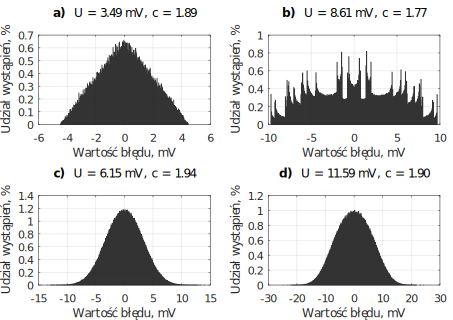
\includegraphics{obrazki/hist_part_a}
\caption{Histogramy błędów \textbf{a)}~statycznego, \textbf{b)}~dynamicznego, \textbf{c)}~losowego, \textbf{d)}~wypadkowego, wielkości wyjściowej zastosowanego w eksperymencie symulacyjnym przetwornika pomiarowego \label{fig_symul_parta_hist}}
\end{center}
\end{figure}

Analizując przedstawiony budżet niepewności oraz związane z nim histogramy zauważyć można, że w analizowanym przypadku nie występuje żaden błąd dominujący. W przypadku błędu statycznego błąd ten ma identyczny rozkład, jak rozkład skorelowanej z nim temperatury. Rozkład błędu dynamicznego wynika ze splotu jego sześciu harmonicznych, o przedstawionych w tabeli \ref{tab_sym_parta_params_dyn_list} parametrach.

W celu weryfikacji zaproponowanej metody i przedstawionego modelu błędu przeprowadzono eksperyment metodą Monte-Carlo, wykonując sto tysięcy powtórzeń wyznaczenia wielkości wyjściowej analizowanego obiektu. Podczas eksperymentu losowano z przedziału $<-2 \pi f_{1};2 \pi f_{1}>\unit{rad}$ fazę początkową sygnału wejściowego, przy czym wylosowanie każdej w możliwych wartości było jednakowo prawdopodobne. Błąd wypadkowy analizowanego obiektu wyznaczano zgodnie z równaniem:
\begin{equation}
e_{a,\Sigma}(t) \label{eqn_sym_parta_error_sum},
\end{equation}
a następnie na jego podstawie opracowano histogram, który posłużył do identyfikacji parametrów rozkładu błędu. Wyznaczona na drodze eksperymentu niepewność $U_{a,\Sigma}$ wyniosła TODO, co pokrywa się z wyznaczoną w równaniu \eqref{eqn_sym_parta_uncert_sum} wartością. Wobec przedstawionych rozważań i przeprowadzonego eksperymentu można stwierdzić, że zaproponowany model błędu odpowiednio opisuje związki pomiędzy kolejnymi błedami, zachodzące w analizowanym obiekcie.


\begin{comment}
\section{Analiza wzmacniacza pomiarowego}



\section{Analiza przetwornika analogowo-cyfrowego}



\section{Analiza algorytmu transformacji falkowej}


\section{Podsumowanie przeprowadzonego eksperymentu}
\end{comment}

